\section{ Ryhmähyppy }
\label{jatkokoulutuksen-suoritukset-ryhmahyppy}


Ryhmähypyillä harjoittelet turvallisen ryhmähyppäämisen perusteita. Suorituksina on hyppyjä oppilaan FS-ohjelmasta (\ref{fs-kuviohyppaaminen-hyppyohjelma} s.\pageref{fs-kuviohyppaaminen-hyppyohjelma}). Myös freehyppyjä voidaan hypätä, jos kouluttajan ja oppilaan taidot riittävät. Olennaista on, että oppilas pystyy näyttämään hallitsevansa kaikki turvallisen ryhmähyppäämisen osa-alueet: 

\begin{itemize}
\item  Toiminta maassa, lentokoneessa ja uloshypyssä. 
\item  Toiminta vapaapudotuksessa, muodostelman lähestyminen ja otteiden ottaminen turvallisesti. 
\item  Purku ja liuku (oikeaan suuntaan ja riittävän tehokkaasti) 
	\begin{itemize}
	\item Purku kahdella ensimmäisellä hypyllä 1800 metrissä, seuraavilla vähintään 1600 metrissä 
	\end{itemize}
\item  Aloita avaustoimenpiteet 1200 metrin korkeudessa. 
\end{itemize}
\begin{itemize}
\item  Kaikkia ryhmähyppyjä yhdistää seuraava toimintajärjestys muodostelmaa lähestyttäessä: 
	\begin{enumerate}[label=\bfseries \arabic*)]
	\item TASO (Level) 
		\begin{itemize}
		\item Lennä samalle tasolle muodostelman kanssa. 
		\end{itemize}
	\item PAIKKA (Slot) 
		\begin{itemize}
		\item Lennä omaan paikkaasi kuvassa. 
		\end{itemize}
	\item OTE (Dock) 
		\begin{itemize}
		\item Ota ote. 
		\end{itemize}
	\end{enumerate}
\end{itemize}
\subsection{ Oppilaan toiminta }
\label{jatkokoulutuksen-suoritukset-oppilaan-toiminta}

\begin{itemize}
\item  UH-harjoittelu, otteet ja ovelle asettautuminen 
\item  Hypyn harjoittelu maassa 
\end{itemize}
\subsection{ Oppimistavoitteet }
\label{jatkokoulutuksen-suoritukset-oppimistavoitteet}

\begin{enumerate}[label=\bfseries \arabic*)]
\item  Toimi turvallisesti vapaassa, kun toteutat harjoiteltua hyppysuunnitelmaa. 
\item  Näytä purkumerkki sovitussa korkeudessa. 
\item  Liu'u oikeaan suuntaan ja tehokkaasti (vähintään 5 sekuntia). 
\item  Avaa sovitussa korkeudessa. 
\end{enumerate}
\subsection{ Hyppylennolla }
\label{jatkokoulutuksen-suoritukset-hyppylennolla}


Mikäli uloshyppy suoritetaan otteilla, sen täytyy olla yhdenaikainen, ja jokaisen hyppääjän tulee heti uloshypyssä päästä ilmavirtaan oikein. Kertaa, miten siirryt ovelle, otat otteet ja miten uloshyppylaskenta tehdään.  

\subsection{ Hypyn kulku }
\label{jatkokoulutuksen-suoritukset-hypyn-kulku}


Keskity omaan suoritukseesi ja säännölliseen korkeuden tarkkailuun. Muista, että turvallinen toiminta on tärkeämpää kuin hyppysuunnitelman onnistuminen. 


\end{multicols}\pagebreak\begin{multicols}{2} 

\section{ Freehyppy }
\label{jatkokoulutuksen-suoritukset-freehyppy}


Freehypyillä hyppäät suorituksia oppilaan freefly-ohjelmasta (\ref{free-hyppaaminen-hyppyohjelma} s.\pageref{free-hyppaaminen-hyppyohjelma}). 

\begin{itemize}
\item  Tutustut freelentämisen alkeisiin. 
\item  Opettelet vartalon hallintaa muussakin asennossa kuin boksissa. 
\end{itemize}
\subsection{ Oppilaan toiminta }
\label{jatkokoulutuksen-suoritukset-oppilaan-toiminta}

\begin{itemize}
\item  Varmista, että käytettävä laskuvarjokalusto on sopiva freekäyttöön. 
\item  Harjoittele asentoa maassa. 
\end{itemize}
\subsection{ Oppimistavoitteet }
\label{jatkokoulutuksen-suoritukset-oppimistavoitteet}

\begin{enumerate}[label=\bfseries \arabic*)]
\item  Tee hyppysuoritus kuten se on harjoiteltu. 
\item  Näytä purkumerkki sovitussa korkeudessa. 
\item  Liu'u oikeaan suuntaan ja tehokkaasti (vähintään 5 sekuntia). 
\item  Avaa sovitussa korkeudessa. 
\end{enumerate}
\subsection{ Hyppylennolla }
\label{jatkokoulutuksen-suoritukset-hyppylennolla}


Mikäli uloshyppy suoritetaan otteilla, sen täytyy olla yhdenaikainen, ja jokaisen hyppääjän tulee heti uloshypyssä päästä ilmavirtaan oikein. Kertaa, miten siirryt ovelle, otat otteet ja miten uloshyppylaskenta tehdään. 

\subsection{ Hypyn kulku }
\label{jatkokoulutuksen-suoritukset-hypyn-kulku}

\begin{itemize}
\item  Keskity omaan suoritukseesi ja säännölliseen korkeuden tarkkailuun. Muista että vapaapudotusnopeus on suurempi kuin mahallaan hypätessä.  
\item  Työskentele niin, että rintamasuuntasi on poikittain hyppykoneen linjaan nähden. 
\item  Mene palloasentoon (\ref{turvallisuus-freehyppaamisessa-palloasento} s.\pageref{turvallisuus-freehyppaamisessa-palloasento}), jos menetät stabiilin asennon. Näin vältät suuren nopeuden muutoksen (korkkaaminen). 
\item  Sovitusta purkukorkeudesta on pidettävä kiinni. 
	\begin{itemize}
	\item  Vaikka hyppäisit yksin, harjoittele purkua. 
	\end{itemize}
\end{itemize}

\end{multicols}\pagebreak\begin{multicols}{2} 

\section{ Kuvunkäsittelyhyppy }
\label{jatkokoulutuksen-suoritukset-kuvunkasittelyhyppy}


Kuvunkäsittelyhypyt on hypättävä ennen muita suorituksia, jos oppilas saa jatkokoulutuksessa luvan käyttää omia varusteita tai kerhon varusteita, joita ei ole hyväksytty alkeis- / peruskoulutuskäyttöön 

\begin{itemize}
\item  Hyppykorkeus on 2000 metriä, josta hypätään 8-10 s vapaa. 
\item  Vapaapudotussuorituksia ei tehdä samalla hypyllä. 
\end{itemize}
\subsection{ Oppilaan toiminta }
\label{jatkokoulutuksen-suoritukset-oppilaan-toiminta}

\begin{itemize}
\item  Käy hyppysuoritus läpi (\ref{kuvunkasittely-oppilaana-kuvunkasittelyhypyt} s.\pageref{kuvunkasittely-oppilaana-kuvunkasittelyhypyt}). 
\item  Tarkasta sääolosuhteet. 
\item  Määritä UH-paikka. (aika varjon varassa pidempi?) 
\end{itemize}
\subsection{ Oppimistavoitteet }
\label{jatkokoulutuksen-suoritukset-oppimistavoitteet}

\begin{itemize}
\item  Oppia käsittelemään varjoa kantohihnoista 
\item  Oppia käsittelemään varjoa eri jarrutustiloissa 
\item  Oppia erilaisia loppuvetotapoja. 
\end{itemize}
\subsection{ Hyppylennolla }
\label{jatkokoulutuksen-suoritukset-hyppylennolla}


Keskity suoritukseen ja varmista oikea uloshyppypaikka, koska avaat tavallista korkeammalla. Varmista muiden pokassa olijoiden tietävän korkean avauksesi. 

\subsection{ Hypyn kulku }
\label{jatkokoulutuksen-suoritukset-hypyn-kulku}


Avauksen jälkeen varmistaudu sijainnistasi, ettet ole liian aikaisin maalialueen päällä. Suorita hyppyyn kuuluvat tehtävät tarkkaillen korkeutta, ilmatilaa sekä sijaintia maalialueeseen nähden. 


\end{multicols}\pagebreak\begin{multicols}{2} 

\section{ Koehyppy }
\label{jatkokoulutuksen-suoritukset-koehyppy}


Koehypyllä oppilas osoittaa hallitsevansa normaalin hyppytilanteen maasta maahan -periaatteella ja olevansa valmis toimimaan itsenäisenä hyppääjänä. 

\subsection{ Oppilaan toiminta }
\label{jatkokoulutuksen-suoritukset-oppilaan-toiminta}


Hän valmistelee pokan kaikilta osin pokan vanhimman roolissa: 

\begin{itemize}
\item  huolehtii varusteistaan 
\item  valitsee ja suunnittelee turvallisen hypyn 
\item  päättää pokassa olevien uloshyppyjärjestyksen 
\item  määrittää UH-paikan ja hyppylinjan koko pokalle tuulitietojen avulla 
\item  katsoo UH-paikan koneesta 
\item  toteuttaa suunnitellun hypyn 
\item  ohjaa varjoaan turvallisesti ja laskeutuu sovitulle alueelle.  
\end{itemize}

Kaikkien osioiden on sujuttava itsenäisesti ilman apua, koska tämän jälkeen hän toimii itsenäisenä hyppääjänä. 

\subsection{ Oppimistavoitteet }
\label{jatkokoulutuksen-suoritukset-oppimistavoitteet}

\begin{enumerate}[label=\bfseries \arabic*)]
\item  Kykenee huolehtimaan itsenäisesti varusteistaan 
\item  Pystyy päättelemään turvallisen uloshyppyjärjestyksen  
\item  Kykenee määrittämään sopivan linjan ja UH-paikan koko pokalle 
\item  Suoriutuu kokemukseensa nähden sopivasta hyppysuorituksesta 
\end{enumerate}
\subsection{ Hyppylennolla }
\label{jatkokoulutuksen-suoritukset-hyppylennolla}

\begin{itemize}
\item  Varmistaa koneen lastauksen oikeassa järjestyksessä 
\item  Määrittää UH-paikan 
\end{itemize}
\subsection{ Hypyn kulku }
\label{jatkokoulutuksen-suoritukset-hypyn-kulku}


Suoritetaan suunniteltu hyppy korkeutta aktiivisesti tarkkaillen. Varjon varassa huomioidaan muut ilmassa olevat hyppääjät ja vältetään ruuhkaa laskeutumisessa. 

\end{multicols}
\pagebreak 
\begin{figure}[t!]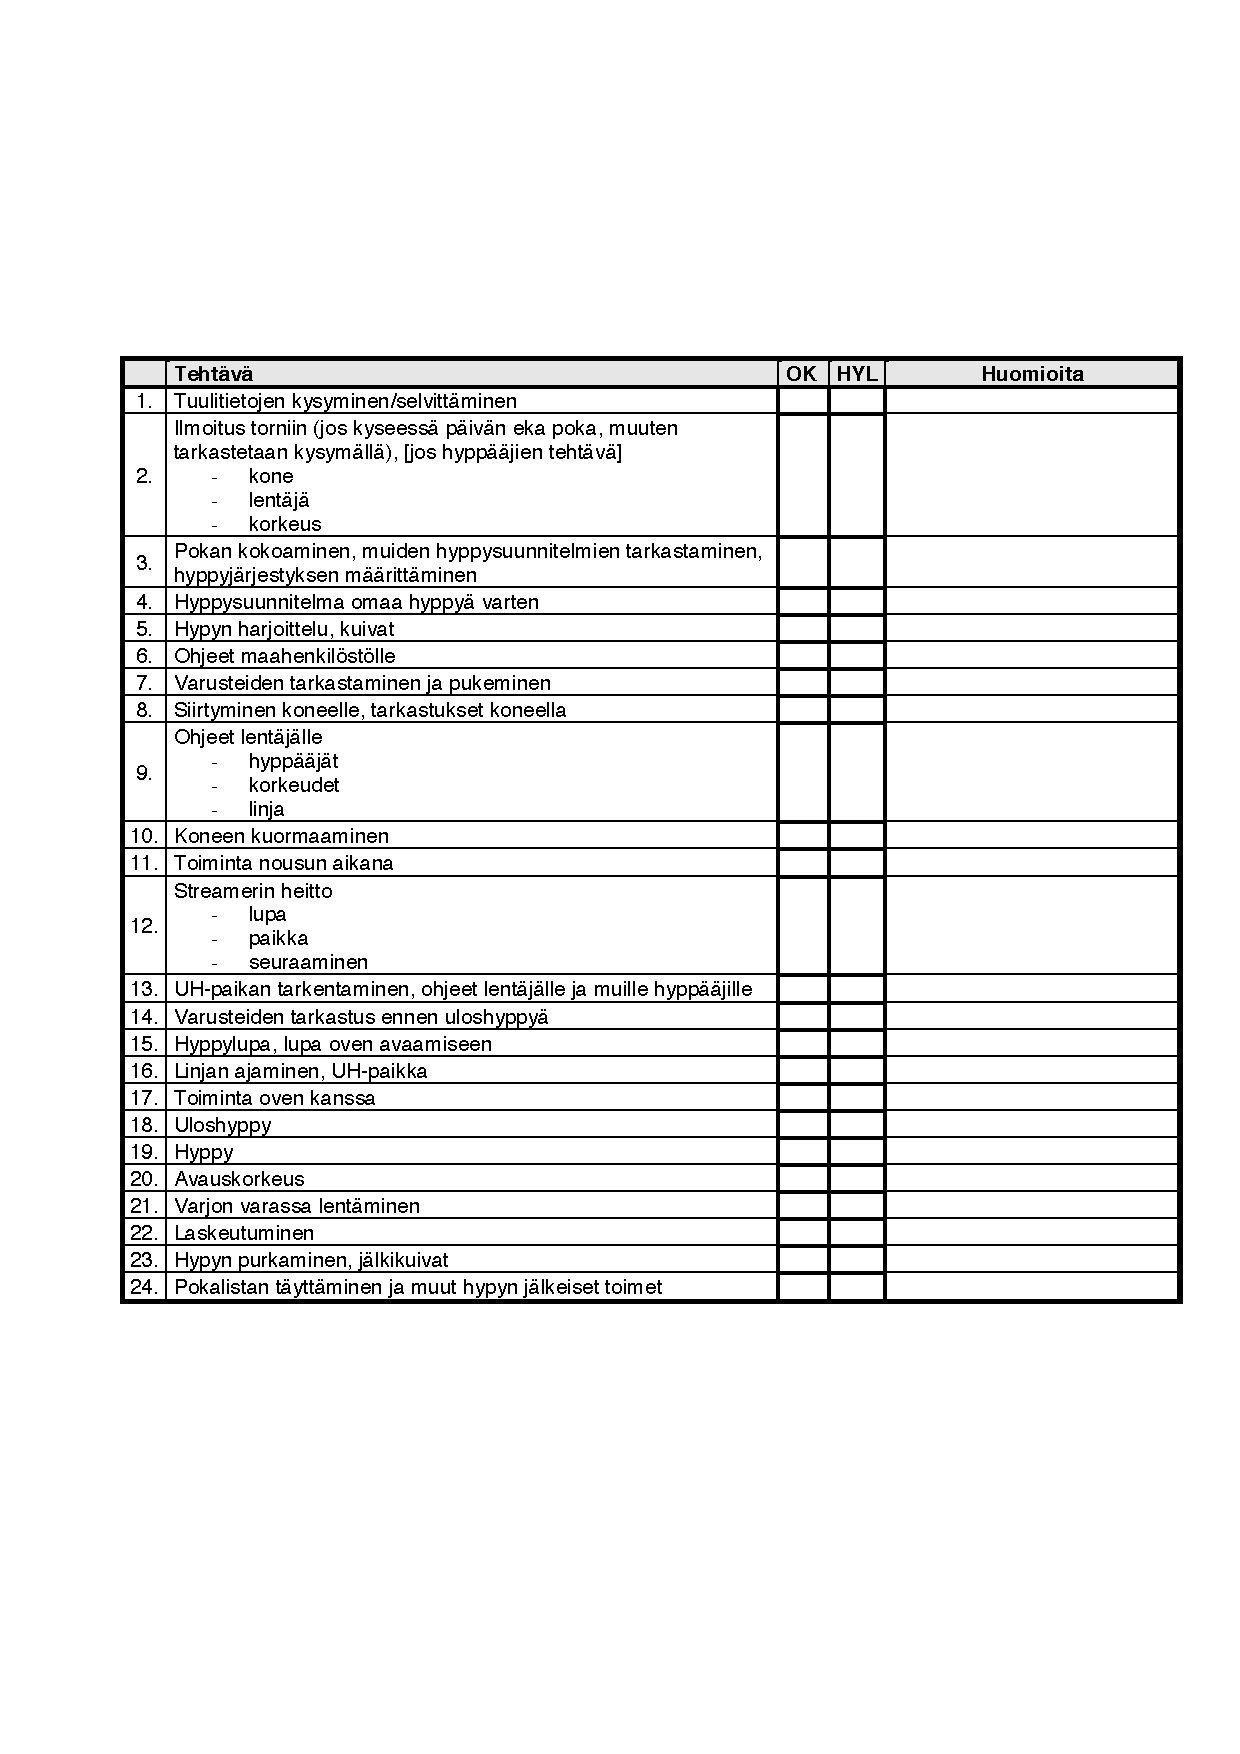
\includegraphics[width=0.95\textwidth]{Koehyppy-lomake.pdf}\caption{Ohjeellinen luettelo koehypyllä huomioitavista asioista}\end{figure} 
\begin{multicols}{2}
